\documentclass[12pt,a4paper]{article}
\usepackage[utf8]{vietnam}
\usepackage{amsmath,amssymb}
\usepackage{tabularx}
\usepackage{tikz}
\usetikzlibrary{calc,arrows.meta}
\usepackage{xcolor}
\usepackage{enumitem}
\usepackage{fancyhdr}
\usepackage[top=1.2cm, bottom=1.2cm, left=1.5cm, right=1.5cm]{geometry}
\usepackage[dethi]{ex_test}
\SAOPTN{widthSA=2.6,heightSA=0.62}

\setlength{\headheight}{15pt}
\setlength{\parskip}{0pt}

% Dòng kẻ chấm mờ chuẩn viết tay
\newcommand{\dongke}[1]{%
  \begingroup%
  \setlength{\parskip}{0pt}%
  \baselineskip=18.5pt%
  \vspace{1.0mm}%
  \foreach \i in {1,...,#1}{%
    \noindent{\color{gray!60}\dotfill}\par%
  }%
  \vspace{0.6mm}%
  \endgroup%
}

\pagestyle{fancy}
\fancyhf{}
\rhead{\textit{Môn Toán 7 -- Đề số 7}}
\lhead{\textit{Bộ đề ôn tập Giữa học kì I}}
\cfoot{\thepage}

\begin{document}

% --- KHUNG TIÊU ĐỀ ĐỀ THI ---
\noindent
\begin{tabularx}{\linewidth}{X r}
\textbf{TRƯỜNG THCS: \dotfill} & \textbf{ĐỀ KIỂM TRA ĐỊNH KỲ GIỮA HỌC KỲ I} \\
\textbf{Họ và tên: \dotfill} & \textbf{NĂM HỌC 2026 -- 2027} \\
\textbf{Lớp: \dotfill \quad SBD: \dotfill} & \textbf{Môn: TOÁN 7} \\
& \textit{Thời gian làm bài: 90 phút (không kể thời gian phát đề)}
\end{tabularx}

\vspace{1.5mm}
\noindent
\begin{tabularx}{\linewidth}{|p{3.5cm}|X|}
\hline
\centering\textbf{Điểm số} & \centering\textbf{Lời nhận xét của thầy cô giáo} \tabularnewline
\rule{0pt}{1.6cm} & \\
\hline
\end{tabularx}

\vspace{2.5mm}
\begin{center}
\textbf{\large ĐỀ SỐ 7}
\end{center}

\noindent\textbf{\large PHẦN I. CÂU TRẮC NGHIỆM NHIỀU PHƯƠNG ÁN LỰA CHỌN (3,0 điểm)}

\textit{Thí sinh trả lời từ câu 1 đến câu 12. Mỗi câu hỏi chỉ chọn một phương án đúng nhất và ghi vào bảng đáp án.}

\vspace{1mm}
\begin{ex}
Trong các số sau, số nào KHÔNG phải là số hữu tỉ?
\choice
{$-\dfrac{5}{6}$}
{$1\dfrac{2}{3}$}
{\True $\dfrac{7}{0}$}
{$-0{,}85$}
\end{ex}

\begin{ex}
Số đối của số hữu tỉ $-\dfrac{3}{8}$ là:
\choice
{\True $\dfrac{3}{8}$}
{$\dfrac{8}{3}$}
{$-\dfrac{3}{8}$}
{$-\dfrac{8}{3}$}
\end{ex}

\begin{ex}
Kết quả của phép tính $5^4 \cdot 5^7$ viết dưới dạng một lũy thừa là:
\choice
{$5^{28}$}
{\True $5^{11}$}
{$25^{11}$}
{$5^3$}
\end{ex}

\begin{ex}
Bỏ dấu ngoặc của biểu thức $A = -(m - n + p - q)$ ta được:
\choice
{$-m - n + p - q$}
{\True $-m + n - p + q$}
{$-m + n + p + q$}
{$-m - n - p - q$}
\end{ex}

\begin{ex}
So sánh hai số hữu tỉ $-0{,}6$ và $-\dfrac{3}{4}$, khẳng định nào sau đây đúng?
\choice
{$-0{,}6 < -\dfrac{3}{4}$}
{$-0{,}6 = -\dfrac{3}{4}$}
{\True $-0{,}6 > -\dfrac{3}{4}$}
{$-0{,}6 \le -\dfrac{3}{4}$}
\end{ex}

\begin{ex}
Căn bậc hai số học của $81$ là:
\choice
{\True $9$}
{$-9$}
{$9$ và $-9$}
{$81$}
\end{ex}

\begin{ex}
Trong các số sau, số nào là số vô tỉ?
\choice
{$\sqrt{25}$}
{$1{,}(3)$}
{\True $\sqrt{5}$}
{$-3{,}14$}
\end{ex}

\begin{ex}
Một hình lăng trụ đứng có diện tích đáy $S = 15\text{ cm}^2$ và chiều cao $h = 8\text{ cm}$. Thể tích $V$ của hình lăng trụ đứng đó là:
\choice
{\True $120\text{ cm}^3$}
{$60\text{ cm}^3$}
{$40\text{ cm}^3$}
{$23\text{ cm}^3$}
\end{ex}

\begin{ex}
Trong định lí: ''Nếu hai đường thẳng phân biệt cùng vuông góc với một đường thẳng thứ ba thì chúng song song với nhau'', phần kết luận là:
\choice
{Hai đường thẳng phân biệt cùng vuông góc với đường thẳng thứ ba}
{\True Chúng song song với nhau}
{Hai đường thẳng vuông góc với nhau}
{Đường thẳng thứ ba vuông góc với hai đường thẳng}
\end{ex}

\begin{ex}
Cho điểm $M$ nằm ngoài đường thẳng $d$. Số đường thẳng đi qua $M$ và song song với $d$ là:
\choice
{$0$}
{\True $1$}
{$2$}
{Vô số}
\end{ex}

\begin{ex}
Cho $a \parallel b$, đường thẳng $c$ cắt cả $a$ và $b$. Biết một góc trong cùng phía có số đo bằng $70^\circ$, số đo của góc trong cùng phía còn lại là:
\choice
{$70^\circ$}
{\True $110^\circ$}
{$180^\circ$}
{$20^\circ$}
\end{ex}

\begin{ex}
Cho $\Delta MNP = \Delta DEF$. Khẳng định nào sau đây là đúng?
\choice
{$MN = DF$}
{$MP = DE$}
{\True $NP = EF$}
{$\widehat{M} = \widehat{E}$}
\end{ex}


\vspace{1mm}
\noindent\textbf{BẢNG TRẢ LỜI TRẮC NGHIỆM PHẦN I:}
\begin{center}
\begin{tabular}{|c|c|c|c|c|c|c|c|c|c|c|c|c|}
\hline
\textbf{Câu} & \textbf{1} & \textbf{2} & \textbf{3} & \textbf{4} & \textbf{5} & \textbf{6} & \textbf{7} & \textbf{8} & \textbf{9} & \textbf{10} & \textbf{11} & \textbf{12} \\
\hline
\textbf{Chọn} & \rule{0pt}{0.65cm} & & & & & & & & & & & \\
\hline
\end{tabular}
\end{center}
\vspace{2mm}

\setcounter{ex}{0}
\noindent\textbf{\large PHẦN II. CÂU TRẮC NGHIỆM ĐÚNG SAI (2,0 điểm)}

\textit{Thí sinh trả lời câu 1 và câu 2. Trong mỗi ý a), b), c), d) ở mỗi câu, thí sinh chọn đúng hoặc sai.}

\vspace{1mm}
\begin{ex}
Cho hai số hữu tỉ $x = -\dfrac{3}{5}$ và $y = \dfrac{2}{3}$. Xét tính đúng sai của các mệnh đề sau:
\choiceTF
{\True Số $x$ là số hữu tỉ âm, số $y$ là số hữu tỉ dương}
{\True Tổng $x + y$ có giá trị bằng $\dfrac{1}{15}$}
{\True Tích $x \cdot y$ có giá trị bằng $-\dfrac{2}{5}$}
{Số đối của $x$ nhỏ hơn số đối của $y$}
\end{ex}

\begin{ex}
Cho hai đường thẳng $a$ và $b$ song song với nhau. Đường thẳng $c$ cắt đường thẳng $a$ tại điểm $A$ và cắt đường thẳng $b$ tại điểm $B$. Biết rằng trong bốn góc tạo thành tại đỉnh $A$, có một góc bằng $60^\circ$. Xét tính đúng sai của các mệnh đề sau:
\choiceTF
{\True Góc kề bù với góc $60^\circ$ tại đỉnh $A$ có số đo bằng $120^\circ$}
{Góc so le trong với góc $60^\circ$ tại đỉnh $B$ có số đo bằng $120^\circ$}
{\True Góc đồng vị với góc $60^\circ$ tại đỉnh $B$ có số đo bằng $60^\circ$}
{\True Hai góc trong cùng phía được tạo bởi đường thẳng $c$ cắt hai đường thẳng $a, b$ có tổng số đo bằng $180^\circ$}
\end{ex}


\noindent\textbf{BẢNG TRẢ LỜI PHẦN II:}
\begin{center}
\begin{tabular}{|c|c|c|c|c||c|c|c|c|c|}
\hline
\textbf{Câu 1} & \textbf{a)} & \textbf{b)} & \textbf{c)} & \textbf{d)} & \textbf{Câu 2} & \textbf{a)} & \textbf{b)} & \textbf{c)} & \textbf{d)} \\
\hline
\textbf{Đ/S} & \rule{0pt}{0.6cm} & & & & \textbf{Đ/S} & & & & \\
\hline
\end{tabular}
\end{center}
\vspace{2mm}

\setcounter{ex}{0}
\noindent\textbf{\large PHẦN III. CÂU HỎI TRẢ LỜI NGẮN (1,0 điểm)}

\textit{Thí sinh trả lời câu 1 và câu 2. Điền kết quả vào ô trống.}

\vspace{1mm}
\begin{ex}
Tìm số hữu tỉ $x$, biết: $\left(x + \dfrac{1}{2}\right)^3 = -\dfrac{1}{27}$. \shortans{$x = -\dfrac{5}{6}$}
\end{ex}

\begin{ex}
Tìm số thực $x$, biết: $|x - 0{,}5| + 0{,}75 = 2{,}25$. \shortans{$x = 2$ hoặc $x = -1$}
\end{ex}


\newpage
\setcounter{ex}{0}
\noindent\textbf{\large PHẦN IV. TỰ LUẬN (4,0 điểm)}

\textit{Thí sinh trình bày chi tiết lời giải vào giấy làm bài.}

\vspace{1mm}
\begin{ex}
Thực hiện phép tính (tính hợp lý nếu có):
\begin{enumerate}[label=\textbf{\alph*)}, leftmargin=0.8cm, itemsep=1pt]
\item $\dfrac{7}{6} - \dfrac{1}{6} + \dfrac{5}{8}$;
\item $-\dfrac{5}{13} \cdot \dfrac{2}{5} + \dfrac{5}{13} \cdot \left(-\dfrac{3}{5}\right)$;
\item $\left[\left(\dfrac{2}{3} - 0{,}25\right) + (-2)^2 \cdot \dfrac{3}{16}\right] - 1$.
\end{enumerate}
\end{ex}
\vspace{1.5mm}

\begin{ex}
Tìm $x$:
\begin{enumerate}[label=\textbf{\alph*)}, leftmargin=0.8cm, itemsep=1pt]
\item $x - \dfrac{1}{9} = -\dfrac{5}{6}$;
\item $-\dfrac{1}{5} + \dfrac{6}{5} : x = (-2)^2$.
\end{enumerate}
\end{ex}
\vspace{1.5mm}

\begin{ex}
\immini{
Cho hình vẽ, biết $\widehat{yOz} = 50^\circ$.
\begin{enumerate}[label=\textbf{\alph*)}, leftmargin=0.8cm, itemsep=1pt]
\item Kể tên các cặp góc kề bù trong hình vẽ.
\item Kẻ $Ot$ là tia phân giác của $\widehat{xOz}$. Tính số đo $\widehat{xOz}$ và $\widehat{xOt}$.
\end{enumerate}
}{
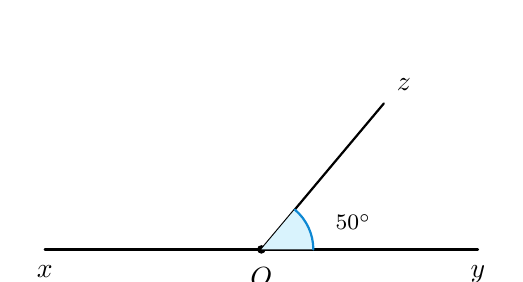
\begin{tikzpicture}[scale=1.1, line cap=round, line join=round]
    \coordinate (O) at (0, 0);
    \coordinate (X) at (-2.5, 0);
    \coordinate (Y) at (2.5, 0);
    \coordinate (Z) at (50:2.2);

    \draw[thick] (X) node[below=2pt] {$x$} -- (Y) node[below=2pt] {$y$};
    \draw[thick] (O) -- (Z) node[above right=1pt] {$z$};

    \filldraw[black] (O) circle (1.2pt) node[below=3pt] {$O$};

    \fill[cyan!15] (O) -- (0:0.6) arc (0:50:0.6) -- cycle;
    \draw[cyan!70!blue, thick] (0:0.6) arc (0:50:0.6);
    \node[font=\footnotesize, right=2pt] at (25:0.75) {$50^\circ$};
\end{tikzpicture}
}
\end{ex}
\vspace{1.5mm}

\begin{ex}
Tìm số hữu tỉ $x$ sao cho:
\[ \dfrac{x + 1}{2023} + \dfrac{x + 2}{2022} = \dfrac{x + 3}{2021} + \dfrac{x + 4}{2020}. \]
\end{ex}
\vspace{1.5mm}


\begin{center}
\rule{4cm}{0.4pt}\\
\textit{--- HẾT ---}
\end{center}
\end{document}
